% !TeX root = skripta-konstitutivni-vztahy-materialu.tex
% !TeX lastmodified = 2019-11-27

\subsection{Tlakové zkoušky pro chloroprenovou gumu s~hysterezí a~závislostí na rychlosti zatěžování}
\begin{figure}[H]
	\centering
	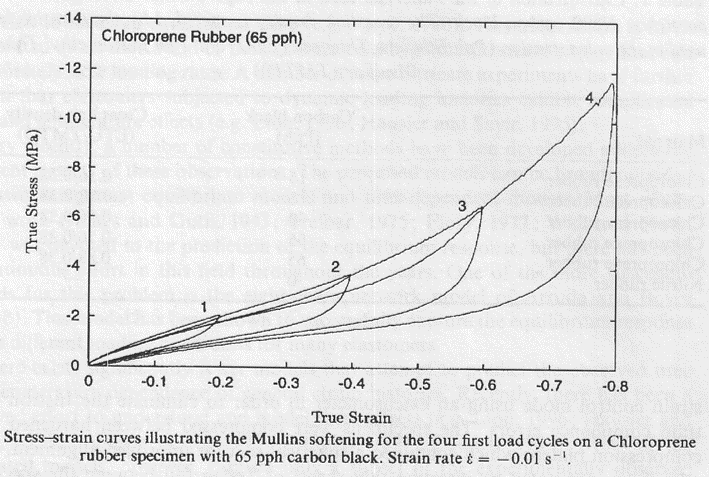
\includegraphics[width=0.7\linewidth]{mullinsovy-efekt-vyrazny}
	\caption{Guma s~velkým obsahem plniva vykazuje významný Mullinsův efekt a~významnou hysterezi (viskoelasticitu).}
	\label{fig:mullinsovy-efekt-vyrazny}
\end{figure}

Mullinsův effekt je změkčení materiálu vlivem předchozího zatížení, při němž dojde k~poškození vzájemných vazeb (zesíťování) mezi vlákny v~materiálu. To se projeví při následujících zatěžovacích cyklech nižší tuhostí materiálu, dokud se nedosáhne maximální hodnoty deformace (deformační energie) z~předchozího zatěžování. Nad touto hodnotou se materiál vrací na tzv. \uv{panenskou} křivku prvního cyklu.

\begin{figure}[H]
	\centering
	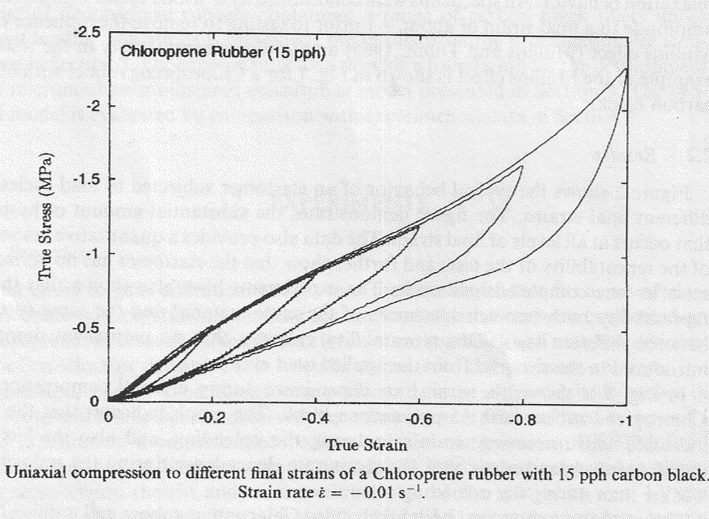
\includegraphics[width=0.7\linewidth]{mullinsovy-efekt-nevyrazny}
	\caption{Guma s~malým množstvím plniva, nepatrným Mullinsovým efektem, ale významnou hysterezí.}
	\label{fig:mullinsovy-efekt-nevyrazny}
\end{figure}

\begin{figure}[H]
	\centering
	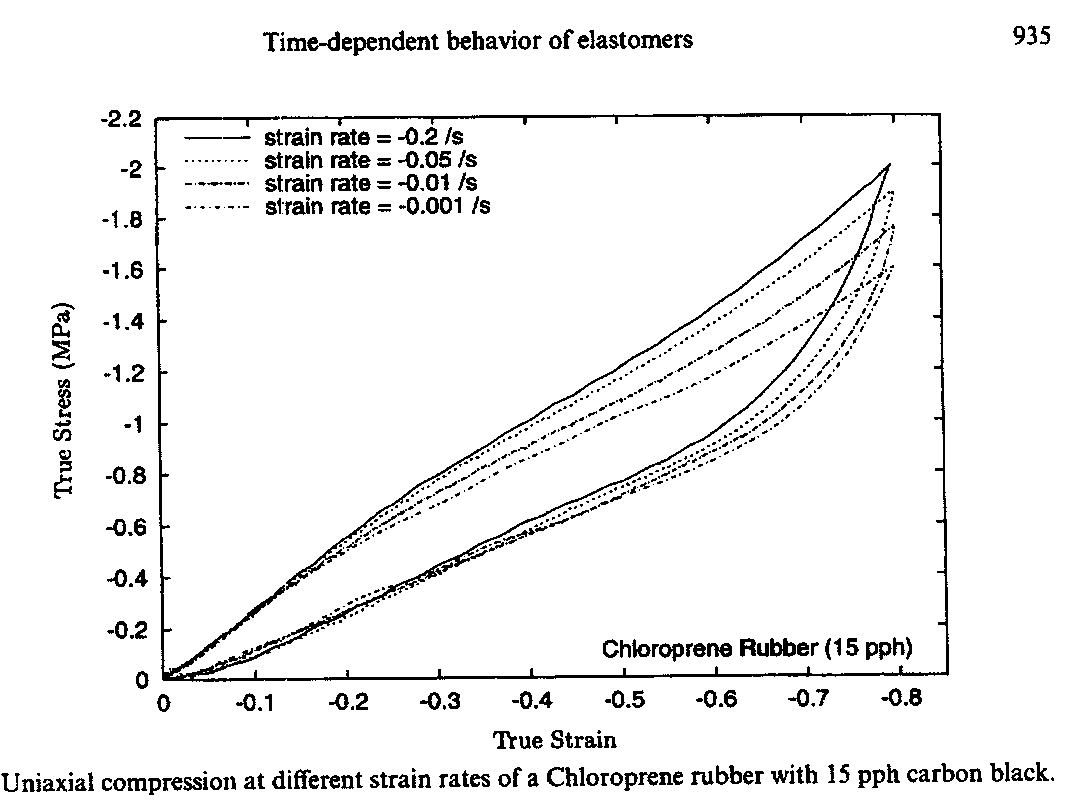
\includegraphics[width=0.7\linewidth]{visko-hyperelasticita}
	\caption{Tlakové zkoušky pro chloroprenovou gumu při různých rychlostech zatěžování -- visko-hyperelasticita}
	\label{fig:visko-hyperelasticita}
\end{figure}
